\section{Simulaciones}

Las simulaciones se realizaron sobre PhoenixSim en una máquina con
las siguientes características:

\begin{table}[H]
\centering
\begin{tabular}{|c|}
\hline
Procesador intel core i7 Ivy Bridge, 3770k. Frecuencia de reloj OC 4.4 GHz \\
4 núcleos - 8 hilos. \\
16 GB de RAM a bus de 1600 MHZ \\
GPU ATI Radeon 5830 \\
128 GB  de disco duro de estado sólido sata3 \\
2 TB de disco duro 7200rpm \\
\hline
\end{tabular}
\caption{Equipo para simulación en PhoenixSim. Codename: mateubuntuSSD}
\label{tb:pcsim3}
\end{table} 

\subsection{Metodología}
En esta fase de la investigación, se planteó realizar la simulación de 
una red de interconexión electrónica y nanofotónica híbrida para 
realizar la comparación del desempeño en términos de latencia y consumo
de energía en 5x2 diferentes escenarios.

Para cada escenario se obtuvo el tamaño de la muestra requerido
para obtener un nivel de confianza del 95\%. Luego se procedió
a definir la comparación para cada variable a medir, 
mediante la prueba de hipótesis para comparación de medias. 

\paragraph{Caso de Estudio} ~\\
La red consta de 2 planos independientes: procesamiento y
red de interconexión fotónica híbrida conmutada. 

El plano de procesamiento está compuesto por 64 
cores en un arreglo de 8x8. 

Como se indica en \cite{dally2004principles}, una red de interconexión está definida
por 3 características principales: la topología empleada, el algoritmo de control de
flujo y el algoritmo de ruteo. La red de interconexión simulada en este experimento
consta de una topología Mesh con concentración de nodos ó C-Mesh (Figura \ref{fig:cmesh}), 
de un algoritmo de control de
flujo llamado \textit{Bubble Flow Control}\cite{puente1999adaptive}\cite{Manual} y
de un algoritmo de enrutamiento basado en un esquema direccionamiento jerárquico
basado en direcciones de la forma $NET.PROC$ como se explica en \cite{Manual}.

\begin{figure}[h!]
\caption{Topología C-Mesh. Fuente: \cite{Manual}}
\centering
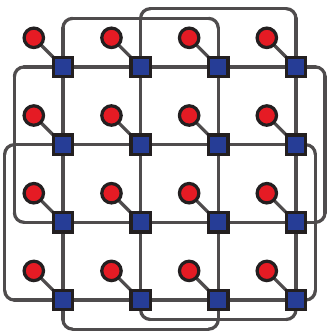
\includegraphics[width=0.5\textwidth,natwidth=333,natheight=336]{figs/cmesh.png}
\label{fig:cmesh}
\end{figure} 

Debido a la topología concentrada que se seleccionó, la red de interconexión 
está compuesta por 4x4 elementos, donde cada nodo terminal da servicio al 
número dado por el parámetro de concentración, que para esta simulación se estableció
en 4.

Sobre cada red se ejecutaron las primeras 5 aplicaciones sintéticas
mencionadas en \ref{sss:synthetic} donde el promedio del tiempo
de generación de mensajes se escogió de 1 milisegundo. Adicionalmente,
para cada red y para cada aplicación, se decidió realizar la simulación
con 2 tamaños de mensajes (pequeño: 512Bytes y grande:65kBites) entre núcleos,
siguiendo la metodología empleada en \cite{hendry2009analysis}.

Algunos de los parámetros de dispositivos fotónicos
empleados en la simulación se muestran en las tablas 
\ref{tb:phpar_wgb} a \ref{tb:phpar_rr}.

\begin{table}[H]
\centering
\begin{tabular}{|c|c|c|}
\hline
Parámetro & Valor & Unidad \\ 
\hline
LatencyRate\_Line & 1.14e-14 &s/$\mu m$ \\
PropagationLoss & 1.5e-4 & dB/um \\
\hline
\end{tabular}
\caption{Parámetros de guía de onda. \cite{xia2006ultracompact} \cite{gnan2008fabrication}}
\label{tb:phpar_wg}
\end{table} 

\begin{table}[H]
\centering
\begin{tabular}{|c|c|c|}
\hline
Parámetro & Valor & Unidad \\ 
\hline
Angle\_Bend & 90 & grados \\
Latency\_Bend & .06e-12 &s \\
BendingLoss & .005 & dB \\
\hline
\end{tabular}
\caption{Parámetros de guía de onda doblada. \cite{xia2006ultracompact}}
\label{tb:phpar_wgb}
\end{table} 

\begin{table}[H]
\centering
\begin{tabular}{|c|c|c|}
\hline
Parámetro & Valor & Unidad \\ 
\hline
CrossingLoss & .15   & dB\\
Crosstalk\_Cross & 40 &dB\\
\hline
\end{tabular}
\caption{Parámetros de cruce de guía de onda. \cite{bogaerts2007low}}
\label{tb:phpar_wgc}
\end{table} 

\begin{table}[H]
\centering
\begin{tabular}{|c|c|c|}
\hline
Parámetro & Valor & Unidad \\ 
\hline
RingOn\_ER\_2x2 & 20 &dB\\
RingOff\_ER\_2x2 & 25 &dB\\
CrossDelay\_2x2 & 4.35e-12 &s\\
BarDelay\_2x2 & 1.25e-12   &s\\
\hline
RingOn\_ER\_1x2 & 20 &dB\\
RingOff\_ER\_1x2 & 25 &dB\\
ThroughDelay\_1x2 & 1.00e-12 &s\\
DropDelay\_1x2 & 4.10e-12 &s\\
\hline
RingThrough\_ER\_Filter1x2 & 25 &dB\\
RingDrop\_ER\_Filter1x2 & 20 &dB\\
ThroughDelay\_Filter1x2 & 0.14e-12 &s\\
DropDelay\_Filter1x2 & 0.34e-12 &s\\
\hline
RingOn\_ER\_1x2NX& 20 &dB\\
RingOff\_ER\_1x2NX & 25 &dB\\
ThroughDelay\_1x2NX & 0.7e-12 &s\\
DropDelay\_1x2NX & 3.8e-12 &s\\
\hline
RingThrough\_ER\_DetectorFilter & 25 &dB\\
RingDrop\_ER\_DetectorFilter & 20 &dB\\
\hline
\end{tabular}
\caption{Parámetros de anillos resonadores.}
\label{tb:phpar_rr}
\end{table} 


\subsection{Resultados}

Para obtener el tamaño de la muestra necesario para una confiabilidad del 
95\% se empleó la siguiente ecuación: 

\begin{equation}
n=\frac{z^2 s^2}{B^2}
\label{eq:muestra}
\end{equation} 

Donde $n$ es el tamaño de la muestra y $s$ la desviación estándar.
El nivel de confianza dado por $z$ se estableció a un valor de 1.96 que corresponde
a un 95\% de confianza. Por último el parámetro $B$ que indica la precisión,
se estableció según la variable a medir. Para el consumo de energía, este valor
fluctúa entre 0.1\% y 0.8\%, mientras que para la latencia se toma en el orden de 
los nanosegundos.

En las tablas de \ref{tb:sn512} a \ref{tb:st65k} se muestran los valores obtenidos en cada simulación
para las variables de consumo de energía y latencia y el valor $n$ obtenido en cada caso:

\begin{table}[H]
\centering
\begin{tabular}{|c|c|c|c|c|}
\hline
 &E&P&E&P\\
\hline
Random-Seed&All Energy $(J)$&All Energy $(J)$&Latency ($\mu$ s)&Latency ($\mu$ s)\\
\hline
6&0.0670822&0.00795576&0.0691798&0.0792249\\
5&0.0671684&0.00795162&0.0683049&0.0779179\\
4&0.0670545&0.00797981&0.0695929&0.0772176\\
2&0.0670536&0.00795009&0.0700826&0.0790122\\
10&0.0670933&0.00796371&0.0681599&0.0778642\\
8&0.0670919&0.00795244&0.0691727&0.0840341\\
\hline
stdev&4.19633E-05&1.13364E-05&0.000739481&0.002480388\\
mean&0.06709065&0.007958905&0.069082133&0.079211817\\
z&1.96&1.96&1.96&1.96\\
p&0.0015&0.0015&0.03&0.03\\
B&0.000100636&1.19384E-05&0.002072464&0.002376355\\
\hline
n&0.667950099&3.463963085&0.48909428&4.185322852\\
\hline
\end{tabular}
\caption{Datos Simulación App: Neighboor, PkgSize: 512B}
\label{tb:sn512}
\end{table}

\begin{table}[H]
\centering
\begin{tabular}{|c|c|c|c|c|}
\hline
 &E&P&E&P\\
\hline
Random-Seed&All Energy $(J)$&All Energy $(J)$&Latency ($\mu$ s)&Latency ($\mu$ s)\\
\hline
6&0.0672651&0.0079509&0.0865564&0.127786\\
5&0.0670529&0.0079602&0.0894102&0.132535\\
4&0.0670557&0.00796118&0.087135&0.132628\\
2&0.0671679&0.00796183&0.0870683&0.132774\\
10&0.0671439&0.00794885&0.0892598&0.133439\\
\hline
stdev&8.81681E-05&6.20164E-06&0.001342664&0.002289528\\
mean&0.0671371&0.007956592&0.08788594&0.1318324\\
z&1.96&1.96&1.96&1.96\\
p&0.0012&0.0012&0.03&0.03\\
B&8.05645E-05&9.54791E-06&0.002636578&0.003954972\\
\hline
n&4.600953054&1.620723506&0.996242993&1.287411017\\
\hline
\end{tabular}
\caption{Datos Simulación App: Random, PkgSize: 512B}
\label{tb:sr512}
\end{table}

\begin{table}[H]
\centering
\begin{tabular}{|c|c|c|c|c|}
\hline
 &E&P&E&P\\
\hline
Random-Seed&All Energy $(J)$&All Energy $(J)$&Latency ($\mu$ s)&Latency ($\mu$ s)\\
\hline
6&0.0671366&0.00795344&0.116493&0.197834\\
5&0.0671364&0.00796231&0.115827&0.20161\\
4&0.0671169&0.00795815&0.115762&0.198954\\
2&0.0670515&0.00795665&0.116925&0.202891\\
10&0.0672859&0.00795283&0.11856&0.205117\\
8&0.0671018&0.0079642&0.11602&0.201612\\
\hline
stdev&7.88881E-05&4.61203E-06&0.001057811&0.002638301\\
mean&0.067138183&0.00795793&0.116597833&0.201336333\\
z&1.96&1.96&1.96&1.96\\
p&0.0012&0.0012&0.03&0.03\\
B&8.05658E-05&9.54952E-06&0.003497935&0.00604009\\
\hline
n&3.68326535&0.896053751&0.351321474&0.732949518\\
\hline
\end{tabular}
\caption{Datos Simulación App: BitReverse, PkgSize: 512B}
\label{tb:sb512}
\end{table}

\begin{table}[H]
\centering
\begin{tabular}{|c|c|c|c|c|}
\hline
 &E&P&E&P\\
\hline
Random-Seed&All Energy $(J)$&All Energy $(J)$&Latency ($\mu$ s)&Latency ($\mu$ s)\\
\hline
6&0.0671167&0.00797317&0.0898645&0.131713\\
5&0.0670928&0.00797042&0.0994328&0.153952\\
4&0.067287&0.00795941&0.0989025&0.15703\\
2&0.0671297&0.00794928&0.0796521&0.111226\\
10&0.0671326&0.00796399&0.097888&0.158137\\
8&0.0670367&0.00795338&0.0888971&0.133294\\
7&0.0673762&0.00798954&0.090947&0.132685\\
\hline
stdev&0.000119549&1.36029E-05&0.007129387&0.017359803\\
mean&0.067167386&0.007965599&0.092226286&0.139719571\\
z&1.96&1.96&1.96&1.96\\
p&0.0015&0.0015&0.095&0.095\\
B&0.000100751&1.19484E-05&0.008761497&0.013273359\\
\hline
n&5.408864344&4.979186199&2.543664501&6.571129653\\
\hline
\end{tabular}
\caption{Datos Simulación App: HotSpot, PkgSize: 512B}
\label{tb:sh512}
\end{table}

\begin{table}[H]
\centering
\begin{tabular}{|c|c|c|c|c|}
\hline
 &E&P&E&P\\
\hline
Random-Seed&All Energy $(J)$&All Energy $(J)$&Latency ($\mu$ s)&Latency ($\mu$ s)\\
\hline
6&0.0671112&0.00794923&0.0736731&0.0837278\\
5&0.0670484&0.00796436&0.0702405&0.0840095\\
4&0.0671063&0.00796425&0.0707252&0.0889056\\
2&0.067085&0.00795086&0.0715833&0.0927564\\
10&0.0670837&0.0079514&0.0709125&0.08952\\
8&0.0670981&0.00794945&0.0704214&0.0836357\\
7&0.0670697&0.00795191&0.0692727&0.0849632\\
\hline
stdev&2.19061E-05&6.77157E-06&0.001382019&0.003603739\\
mean&0.067086057&0.007954494&0.070975529&0.086788314\\
z&1.96&1.96&1.96&1.96\\
p&0.001&0.001&0.035&0.035\\
B&6.70861E-05&7.95449E-06&0.002484144&0.003037591\\
\hline
n&0.409615903&2.783977714&1.189014215&5.40704914\\
\hline
\end{tabular}
\caption{Datos Simulación App: Tornado, PkgSize: 512B}
\label{tb:st512}
\end{table}


\begin{table}[H]
\centering
\begin{tabular}{|c|c|c|c|c|}
\hline
 &E&P&E&P\\
\hline
Random-Seed&All Energy $(J)$&All Energy $(J)$&Latency ($\mu$ s)&Latency ($\mu$ s)\\
\hline
6&0.0673445&0.00799389&1.51514&0.51567\\
5&0.0671345&0.00799492&1.51138&0.528793\\
4&0.0671509&0.00799738&1.50786&0.522043\\
2&0.0672506&0.00800407&1.50719&0.534181\\
\hline
stdev&9.75049E-05&4.57715E-06&0.003659849&0.008048858\\
mean&0.067220125&0.007997565&1.5103925&0.52517175\\
z&1.96&1.96&1.96&1.96\\
p&0.0015&0.0015&0.03&0.03\\
B&0.00010083&1.19963E-05&0.045311775&0.015755153\\
\hline
n&3.59239214&0.559247838&0.025062029&1.002618005\\
\hline
\end{tabular}
\caption{Datos Simulación App: Random, PkgSize: 65536B}
\label{tb:sr65k}
\end{table}


\begin{table}[H]
\centering
\begin{tabular}{|c|c|c|c|c|}
\hline
 &E&P&E&P\\
\hline
Random-Seed&All Energy $(J)$&All Energy $(J)$&Latency ($\mu$ s)&Latency ($\mu$ s)\\
\hline
6&0.0671338&0.00797883&1.39792&0.328061\\
5&0.0672169&0.0080181&1.39465&0.322767\\
4&0.0671059&0.00797706&1.40607&0.312189\\
2&&0.00798905&&0.323677\\
10&&0.00800833&&0.337259\\
8&&0.00798299&&0.311023\\
\hline
stdev&5.77423E-05&1.69321E-05&0.00588121&0.009881777\\
mean&0.0671522&0.007992393&1.399546667&0.322496\\
z&1.96&1.96&1.96&1.96\\
p&0.0017&0.0017&0.03&0.03\\
B&0.000114159&1.35871E-05&0.0419864&0.00967488\\
\hline
n&0.982837116&5.966009944&0.075375164&4.007661738\\
\hline
\end{tabular}
\caption{Datos Simulación App: Neighboor, PkgSize: 65536B}
\label{tb:sn65k}
\end{table}


\begin{table}[H]
\centering
\begin{tabular}{|c|c|c|c|c|}
\hline
 &E&P&E&P\\
\hline
Random-Seed&All Energy $(J)$&All Energy $(J)$&Latency ($\mu$ s)&Latency ($\mu$ s)\\
\hline
6&0.0672625&0.00799928&1.55446&0.611643\\
5&0.0672618&0.00801075&1.55022&0.605117\\
4&0.0672407&0.00799567&1.55219&0.610232\\
2&0.0671883&0.00800271&1.55416&0.615228\\
\hline
stdev&3.48504E-05&6.44184E-06&0.001968627&0.004191135\\
mean&0.067238325&0.008002103&1.5527575&0.610555\\
z&1.96&1.96&1.96&1.96\\
p&0.001&0.001&0.007&0.007\\
B&6.72383E-05&8.0021E-06&0.010869303&0.004273885\\
\hline
n&1.032032731&2.489566182&0.126018875&3.69428032\\
\hline
\end{tabular}
\caption{Datos Simulación App: BitReverse, PkgSize: 65536B}
\label{tb:sb65k}
\end{table}


\begin{table}[H]
\centering
\begin{tabular}{|c|c|c|c|c|}
\hline
 &E&P&E&P\\
\hline
Random-Seed&All Energy $(J)$&All Energy $(J)$&Latency ($\mu$ s)&Latency ($\mu$ s)\\
\hline
6&0.0671994&0.007995&1.56549&0.52534\\
5&0.0671903&0.00800166&1.59177&0.550099\\
4&0.067383&0.00803194&1.59952&0.571698\\
2&0.067201&0.00799349&1.56815&0.502018\\
10&0.0672379&0.00800522&1.59104&0.554626\\
8&0.0671213&0.00800309&1.58954&0.526473\\
7&0.0674615&0.00801929&1.57188&0.525672\\
\hline
stdev&0.000120675&1.38231E-05&0.013577873&0.023394081\\
mean&0.067256343&0.008007099&1.582484286&0.536560857\\
z&1.96&1.96&1.96&1.96\\
p&0.0014&0.0014&0.035&0.035\\
B&9.41589E-05&1.12099E-05&0.05538695&0.01877963\\
\hline
n&6.30995691&5.841412563&0.230866389&5.96142471\\
\hline
\end{tabular}
\caption{Datos Simulación App: HotSpot, PkgSize: 65536B}
\label{tb:sh65k}
\end{table}


\begin{table}[H]
\centering
\begin{tabular}{|c|c|c|c|c|}
\hline
 &E&P&E&P\\
\hline
Random-Seed&All Energy $(J)$&All Energy $(J)$&Latency ($\mu$ s)&Latency ($\mu$ s)\\
\hline
6&0.0671693&0.00798253&1.44903&0.373905\\
5&0.0671009&0.00799408&1.42758&0.404685\\
4&0.0671575&0.00800383&1.44217&0.377759\\
2&0.067091&0.00798413&1.43348&0.384779\\
10&0.0671379&0.00799219&1.43278&0.398339\\
8&0.0671538&0.00798319&1.43929&0.388029\\
7&0.0670885&0.00798815&1.43149&0.390422\\
\hline
stdev&3.41615E-05&7.66216E-06&0.007354642&0.010836262\\
mean&0.067128414&0.007989729&1.436545714&0.388274\\
z&1.96&1.96&1.96&1.96\\
p&0.0008&0.0008&0.025&0.025\\
B&5.37027E-05&6.39178E-06&0.035913643&0.00970685\\
\hline
n&1.554509071&5.520398642&0.161107709&4.787563253\\
\hline
\end{tabular}
\caption{Datos Simulación App: Tornado, PkgSize: 65536B}
\label{tb:st65k}
\end{table}

Una vez ejecutadas las simulaciones, se realizaron pruebas hipótesis de diferencia
de medias de la tabla \ref{tb:mvi} para validar o no la hipótesis de que la 
red de interconexión nanofotónicas híbridas con topología P-Mesh es mejor
que su equivalente electrónica E-Mesh.
Las variables que se utilizaron como indicador 
de un mejor sistema fueron el consumo de energía y la latencia del sistema.


\begin{table}[H]
\centering
\begin{tabular}{|c|c|c|c|}
\hline
Caso & Hipótesis & Estadístico de Prueba & Criterio de Rechazo \\
\hline 
$\sigma_1^2 = \sigma_2^2$ &
\specialcell{
    $H_0:\mu_1 = \mu_2$ \\
    $H_A:\mu_1 > \mu_2$ 
} &
\specialcell{
    $S_p = \sqrt{\frac{(n_1-1)S_1^2 + (n_2-1)S_2^2}{n_1+n_2-2}}$ \\ \\
    $t_0=\frac{\hat{x_1} - \hat{x_2}}{S_p\sqrt{\frac{1}{n_1}+\frac{1}{n_2}}} $ \\ \\
    $v= n_1 + n_2 - 2$
}& 
$t_0 > t_{\alpha,v}$ 
\\ 
\hline
$\sigma_1^2 \not= \sigma_2^2$ &
\specialcell{
    $H_0:\mu_1 = \mu_2$ \\
    $H_A:\mu_1 > \mu_2$ 
} &
\specialcell{
    $t_0=\frac{\hat{x_1} - \hat{x_2}}{S_p\sqrt{\frac{S_1^2}{n_1}+\frac{S_2^2}{n_2}}} $ \\ \\
    $v= \frac{ (\frac{S_1^2}{n_1} -  \frac{S_2^2}{n_2}) }
	     {\frac{(\frac{S_1^2}{n_1})^2}{n_1-1} + \frac{(\frac{S_2^2}{n_2})^2}{n_2-1}} $
}& 
$t_0 > t_{\alpha,v}$ 
\\ 
\hline
\end{tabular}
\caption{Estadísticos para Diferencia de Medias. Fuente: \cite{gutierrez2003analisis} }
\label{tb:mvi}
\end{table} 

Según el $n$ obtenido para cada caso en las tablas \ref{tb:sn512} a \ref{tb:st65k}, 
se procedió a realizar el análisis de las 5 aplicaciones
en 2 subgrupos según el tamaño de los mensajes enviados en cada momento.
Adicionalmente, en cada caso, se hizo un analisis de varianza \cite{trejos2004} 
para saber cual de las 2 fórmulas de \ref{tb:mvi} utilizar.

Como el nivel de confianza realizado para la prueba de hipótesis fue del 0.95,
se tiene un valor de $\alpha$ = 0.05. Por lo tanto sólo las pruebas que presenten un valor
inferior a alfa en el valor P se podrá decir con una confiabilidad del 95\% que la
red nanofotónica híbrida es mejor en alguna de las 2 variables que la electrónica.

La prueba de hipótesis y la alterna para las 2 variables de medición se puede ver en la 
tabla \ref{tb:h0ha}. En ambos casos, se busca rechazar la $H_0$, 
es decir confirmar que la red nanofotónica híbrida
se comporta mejor en términos de consumo de energía o lantencia que la electrónica. 


\begin{table}[H]
\centering
\begin{tabular}{|c|c|c|}
\hline
$H_0$ & $H_a$ & Variable\\ 
\hline
$CE_E = CE_P$ & $CE_E > CE_P$ & Consumo de Energía (CE) \\
\hline
$L_E = L_P$ & $L_E > L_P$ & Latencia (L) \\
\hline
\end{tabular}
\caption{My caption here}
\label{tb:h0ha}
\end{table} 

\subsubsection{Paquetes Pequeños (512B)}

En las tablas \ref{tb:eall512} y \ref{tb:lall512} se sintetizan 
las medias del consumo de energía y de
latencia para los mensajes pequeños.

\begin{table}[H]
\centering
\begin{tabular}{|c|c|c|c|}
\hline
&Electrónica&Híbrida Fotónica\\
\hline
Neighboor&0.06709065&0.007958905\\
Random&0.0671371&0.007956592\\
BitReverse&0.067138183&0.00795793\\
HotSpot&0.067167386&0.007965599\\
Tornado&0.067086057&0.007954494\\
\hline
\end{tabular}
\caption{Datos promedio Consumo de Energía $(J)$, PkgSize: 512B}
\label{tb:eall512}
\end{table}


\begin{table}[H]
\centering
\begin{tabular}{|c|c|c|c|}
\hline
&Electrónica&Híbrida Fotónica\\
\hline
Neighboor&0.069082133&0.079211817\\
Random&0.08788594&0.1318324\\
BitReverse&0.116597833&0.201336333\\
HotSpot&0.092226286&0.139719571\\
Tornado&0.070975529&0.086788314\\
\hline
\end{tabular}
\caption{Datos promedio Latencia $(\mu s)$, PkgSize: 512B}
\label{tb:lall512}
\end{table}

Se puede observar gráficamente que el consumo de energía de la red
nanofotónica híbrida es mucho menor que el de la red netamente electrónica.
Sin embargo, la variable de latencia muestra que para este tipo de mensajes
la red fotónica híbrida se comporta peor que la red electrónica.

\begin{figure}[H]
\caption{Comparación Consumo de Energía, PkgSize: 512B. Fuente: Autor.}
\centering
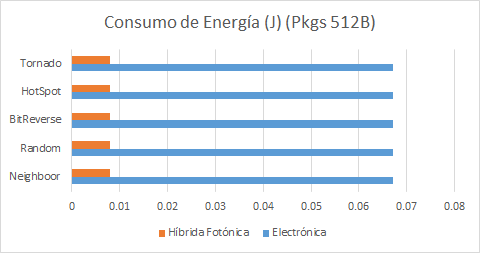
\includegraphics[width=1.0\textwidth,natwidth=483,natheight=256]{figs/E512.png}
\label{fig:e512}
\end{figure} 

\begin{figure}[H]
\caption{Comparación Latencia, PkgSize: 512B. Fuente: Autor.}
\centering
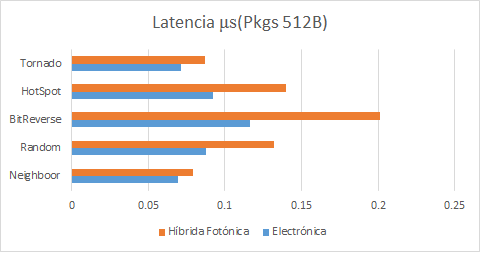
\includegraphics[width=1.0\textwidth,natwidth=483,natheight=256]{figs/L512.png}
\label{fig:l512}
\end{figure} 

Los resultados de las pruebas de hipótesis se presentan a continuación:
 
\begin{table}[H]
\centering
\begin{tabular}{|c|c|c|c|}
\hline
&Valor P&Rechaza $H_0$ ?\\
\hline
Neighboor&7.29052E-32&TRUE\\
Random&2.21789E-23&TRUE\\
BitReverse&2.85143E-29&TRUE\\
HotSpot&1.42176E-32&TRUE\\
Tornado&3.3077E-41&TRUE\\
\hline
\end{tabular}
\caption{Resultados Prueba Hipótesis para la variable Consumo de Energía, PkgSize: 512B}
\label{tb:ettest512}
\end{table}

En la tabla \ref{tb:ettest512} se encontró que en todos los casos se presentó una
respuesta positiva. Esto se puede concluir debido a que el valor P para
en todos los resultados fue mayor a 0.05 y por lo tanto se puede concluir que 
la red nanofotónica híbrida sí es mejor en términos de consumo de potencia
que la red electrónica analizada para tamaños de mensajes pequeños.


\begin{table}[H]
\centering
\begin{tabular}{|c|c|c|c|}
\hline
&Valor P&Rechaza $H_0$ ?\\
\hline
Neighboor&0.99999883&FALSE\\
Random&1&FALSE\\
BitReverse&1&FALSE\\
HotSpot&0.999989&FALSE\\
Tornado&0.9999999&FALSE\\
\hline
\end{tabular}
\caption{Resultados Prueba Hipótesis para la variable Latencia, PkgSize: 512B}
\label{tb:lttest512}
\end{table}

En la tabla \ref{tb:lttest512} se puede confirmar lo observado
gráficamente para la variable de 
latencia. En los paquetes de mensajes pequeños,
no hay evidencias suficientes para afirmar que la red fotónica
es mejor que la electrónica. Es más, en todos los casos se comportó peor.

Este resultado se puede entender desde el punto de vista de la red híbrida,
ya que al necesitar un subplano de control electrónico para hacer el \textit{setup} del
camino antes de enviar los datos por el subplano fotónico. Cuando los mensajes son
pequeños, el sobrecosto de realizar este trabajo sobrepasa en gran medida el 
beneficio de tener una red de transmisión fotónica \cite{shacham2008photonic} y por lo tanto no
logra el rendimiento esperado.

\subsubsection{Tamaño de Paquetes Grande (65kB)}

En las tablas \ref{tb:eall65k} y \ref{tb:lall65k} se sintetizan 
las medias del consumo de energía y de
latencia para los mensajes grandes (65kB).

\begin{table}[H]
\centering
\begin{tabular}{|c|c|c|c|}
\hline
&Electrónica&Híbrida Fotónica\\
\hline
Neighboor&0.0671522&0.007992393\\
Random&0.067220125&0.007997565\\
BitReverse&0.067238325&0.008002103\\
HotSpot&0.067256343&0.008007099\\
Tornado&0.067128414&0.007989729\\
\hline
\end{tabular}
\caption{Datos promedio Consumo de Energía $(J)$, PkgSize: 65kB}
\label{tb:eall65k}
\end{table}


\begin{table}[H]
\centering
\begin{tabular}{|c|c|c|c|}
\hline
&Electrónica&Híbrida Fotónica\\
\hline
Neighboor&1.399546667&0.322496\\
Random&1.5103925&0.52517175\\
BitReverse&1.5527575&0.610555\\
HotSpot&1.582484286&0.536560857\\
Tornado&1.436545714&0.388274\\
\hline
\end{tabular}
\caption{Datos promedio Latencia $(\mu s)$, PkgSize: 65kB}
\label{tb:lall65k}
\end{table}

Nuevamente se puede observar gráficamente que el consumo de energía de la red
nanofotónica híbrida es mucho menor que el de la red netamente electrónica.
Sin embargo, en este caso, la variable de latencia SI muestra que 
para este tipo de mensajes la red fotónica híbrida se comporta mucho mejor 
que la red electrónica.

\begin{figure}[H]
\caption{Comparación Consumo de Energía, PkgSize: 65kB. Fuente: Autor.}
\centering
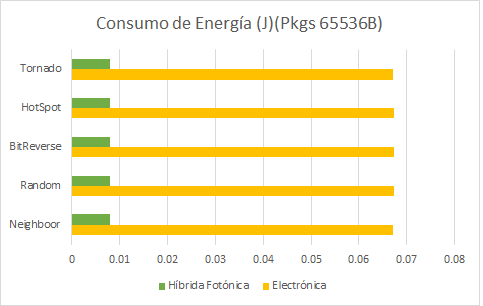
\includegraphics[width=1.0\textwidth,natwidth=483,natheight=306]{figs/E65k.png}
\label{fig:e65k}
\end{figure} 

\begin{figure}[H]
\caption{Comparación Latencia, PkgSize: 65kB. Fuente: Autor.}
\centering
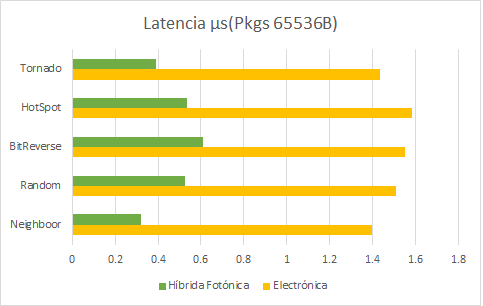
\includegraphics[width=1.0\textwidth,natwidth=483,natheight=306]{figs/L65k.png}
\label{fig:l65k}
\end{figure} 

\begin{table}[H]
\centering
\begin{tabular}{|c|c|c|c|}
\hline
&Valor P&Rechaza $H_0$ ?\\
\hline
Neighboor&2.427440e-22 TRUE&TRUE\\
Random&1.05729E-17&TRUE\\
BitReverse&2.41872E-20&TRUE\\
HotSpot&1.57746E-32&TRUE\\
Tornado&5.3047E-39&TRUE\\
\hline
\end{tabular}
\caption{Resultados Prueba Hipótesis para la variable Consumo de Energía, PkgSize: 65kB}
\label{tb:ettest65k}
\end{table}

En la tabla \ref{tb:ettest65k} se puede observar en todos los casos una
respuesta positiva debido a que el valor P para
todos los resultados fue mayor a 0.05. Por lo tanto, también se puede concluir que 
la red nanofotónica híbrida sí es mejor en términos de consumo de potencia
que la red electrónica analizada para tamaños de mensajes grandes.

\begin{table}[H]
\centering
\begin{tabular}{|c|c|c|c|}
\hline
&Valor P&Rechaza $H_0$ ?\\
\hline
Neighboor&7.08709E-14&TRUE\\
Random&5.37024E-10&TRUE\\
BitReverse&3.01947E-11&TRUE\\
HotSpot&2.99509E-16&TRUE\\
Tornado&8.35414E-21&TRUE\\
\hline
\end{tabular}
\caption{Resultados Prueba Hipótesis para la variable Latencia, PkgSize: 65kB}
\label{tb:lttest65k}
\end{table}

En la tabla \ref{tb:lttest65k} también se encontró en todos los casos una
respuesta positiva. Es decir que para tamaños de mensajes grandes, el sobrecosto
de la subred de control es insignificante en cuanto a las mejoras obtenidas
en latencia por el subplano fotónico de transmisión de datos.


Se pueden observar diferencias en cuanto al valor teórico esperado en las
condiciones de resonancia para todas las simulaciones,
debido a que se asumió que el anillo no presentaba pérdidas $(\alpha = 1)$ en
el cálculo teórico de la transmitancia.

Sin embargo, la que más difiere de todas inclusive en el FSR esperado 
es la simulación mostrada en la figura \ref{fig:meep_res_n}. Esto se puede deber a
que esta simulación se realizó sólamente en 2 dimensiones y por lo tanto
deja de lado la interacción de la onda con el materia de Sílica SiO2.


\subsection{Conclusiones y Trabajos Futuros}
\begin{itemize}
\item Las frecuencias de resonancia del anillo pueden ser manipuladas mediante
modificaciones en el diámetro del anillo, el gap o el índice de refracción. Este
último es de gran importancia por ser la base del funcionamiento algunos dispositivos
moduladores en Silicon Photonics donde se aplica un campo
magnético, generando un efecto plasmónico que altera el índice y por lo tanto
los modos de resonancia.
\item Debido a que se asumió que el anillo no presentaba pérdidas $(\alpha = 1)$ en
el cálculo teórico de la transmitancia tanto del filtro Notch como del filtro
AddDrop, se pueden apreciar diferencias en las condiciones de resonancia
de la teoría con respecto a lo obtenido en la práctica.
\item Las diferencias en el $FSR$ obtenido en las simulaciones realizadas en Meep
con respecto a las realizadas en Lumerical, pueden ser explicadas debido a la 
diferencia en las dimensiones de ambas simulaciones. Mientras que en Lumerical 
se realizó una simulación 3D de ambos filtros, en Meep la mayoría fueron realizadas
en 2D a diferencia del último caso. Este escenario permitió corroborar esta teoría
ya que la simulación Meep 3D del filtro Notch fue muy similar a la simulación del mismo
filtro en la plataforma Lumerical.
\item Como trabajo futuro se plantea realizar nuevas simulaciones para los dos
filtros modificando el diámetro del anillo para visualizar 
la alteración en el FSR y su uso como filtro selectivo o filtro de banda ancha.
\item Se propone también, para un diámetro fijo, realizar simulaciones alterando 
el índice de refracción del anillo para simular el efecto plasmónico que 
sucede dentro del modulador y que hace que se desplacen las frecuencias de resonancia
de un estado On a Off.
\end{itemize} 

